%%%%%%%%%%%%%%%%%%%%%%%%%%%%%%%%%%%%%%%%%%%%%%%%%%%%
\documentclass[fleqn,10pt,twocolumn]{AROB}

\usepackage[utf8]{inputenc}
\usepackage{amsmath}
\usepackage{xeCJK}
\usepackage{svg}
\setCJKmainfont{Hiragino Mincho ProN}

\title{Blood Pressure Estimation Based on Asymmetric Sine Wave Model\\
Residuals Optimized for PPG in 30fps Visible Camera Environment}

\author{Yusuke Nakazawa${}^{1\dagger}$, Kent Nagumo${}^{1}$, Akio Nozawa${}^{1}$}
% The dagger symbol indicates the presenter.
\speaker{Yusuke Nakazawa}

\affils{${}^{1}$Department of Electrical and Electronic Engineering, Graduate School of Science and Engineering, Aoyama Gakuin University\\
(Tel: 080-5326-3916; E-mail: nynynakazawa@gmail.com)\\
}

\abstract{%
We propose a novel blood pressure estimation method for pseudo-PPG signals from smartphone visible cameras that does not rely on frequency decomposition. At a low sampling rate of 30\,fps, conventional frequency-based approaches struggle to extract high-order harmonics accurately. This study adopts the morphological feature approach RTBP (RealTimeBloodPressure) as a baseline and compares two newly proposed methods. The first, sinBP(M), uses the asymmetric sine wave fit parameters (amplitude, phase, mean) directly as regression features. The second, sinBP(D), augments RTBP features with the model residual (distortion index $E$) derived from a physiologically motivated asymmetric sine wave model. Both sinBP(M) and sinBP(D) capture essential waveform characteristics and provide stable blood pressure estimation with reduced noise sensitivity. This study compares RTBP, sinBP(M), and sinBP(D) against a clinical-grade continuous blood pressure monitor in a 30\,fps visible-camera rPPG environment and demonstrates the superiority of the proposed methods.
}

\keywords{%
Blood pressure estimation, Photoplethysmography, Smartphone, Asymmetric sine wave model, Distortion index
}

\begin{document}

\maketitle

%-----------------------------------------------------------------------

\section{Introduction}

Continuous non-invasive blood pressure monitoring is essential for the early detection and management of cardiovascular diseases \cite{ref1,ref2}. In recent years, photoplethysmography (PPG) obtained from smartphone visible cameras has attracted attention as a simple, non-invasive blood pressure estimation modality \cite{ref3}.

PPG waveform features reflect underlying vascular physiology. Amplitude ($A$) indicates vascular distensibility and stroke volume \cite{ref3,ref4}, while peak interval reflects autonomic activity. Relative time-to-peak (TTP), the ratio of peak arrival time to the pulse period, captures earlier reflected-wave return in stiffer vessels and serves as an arteriosclerosis indicator \cite{ref5,ref6}. A linear relationship between these PPG features and blood pressure has been established \cite{ref5,ref7,ref8}. Conventional approaches extract such features via morphological analysis (peaks, TTP) \cite{ref5}, frequency analysis (FFT) \cite{ref9}, or machine learning (deep learning) \cite{ref10}.

However, standard smartphone cameras typically operate at 30\,fps, which is insufficient for precise pulse-wave analysis, and they are susceptible to illumination fluctuations and motion artifacts. Under these conditions, morphological features that depend on fine timing (peak positions, TTP) become unstable, and frequency analysis is constrained by the low sampling rate \cite{ref11,ref12}.

To address these limitations, this study focuses on the overall waveform shape rather than local feature points or frequency components. The overall waveform shape changes depending on blood pressure. We hypothesize that fitting a model function to all data points within one beat smooths out local noise and sampling jitter, enabling robust feature extraction even in a 30\,fps, high-noise environment.

We propose an asymmetric sine wave model that accounts for the asymmetry between the systolic and diastolic phases. Gamma, Beta, and skewed-Gaussian models have been reported for PPG representation \cite{ref13,ref14}, but they require many parameters, incur high computational costs, and are noise-sensitive at low sampling rates. In contrast, the proposed model captures the steep rise and gradual decay characteristic of PPG using the systolic-to-diastolic time ratio ($\alpha$). With only four parameters (amplitude, phase, mean, $\alpha$), the model captures the main waveform features at low computational cost and remains robust at 30\,fps.

The objective of this study is to verify the effectiveness of this asymmetric sine wave model. We examined the following three methods.
(1) RTBP (Baseline): Morphological features (amplitude, heart rate, relative TTP) \cite{ref5}.
(2) Proposed method (Asymmetric sine wave model):
(2-1) sinBP(M): Parameters obtained by fitting the asymmetric sine wave model (amplitude, phase, mean) used directly as features.
(2-2) sinBP(D): RTBP features augmented with the model residual (distortion index $E$) and vascular stiffness index ($E\sqrt{A}$).

All methods employ Ridge regression to handle multicollinearity \cite{ref15}.

The main contribution is an ``asymmetric sine wave model fitting method'' that enables stable feature extraction even in a low-quality 30\,fps video environment. Unlike RTBP, which relies on point measurements, this approach exploits the entire waveform shape, enhancing robustness to noise.

%-----------------------------------------------------------------------

\section{Methods}

\subsection{Asymmetric Sine Wave Model}
The PPG waveform exhibits asymmetry: the systolic (rising) phase is short, whereas the diastolic (falling) phase is long \cite{ref16}. We fit an asymmetric sine wave model $s(t)$ to the measured waveform $x[n]$ via least squares. The model represents the systolic and diastolic phases with sine waves of different effective frequencies (Eq.\,\ref{eq:asymmetric_model}).

\begin{equation}
s(t) = \text{mean} + \frac{A}{2} \cdot \sin(\theta(t))
\label{eq:asymmetric_model}
\end{equation}

\begin{equation}
\theta(t) = \begin{cases}
-\dfrac{\pi}{2} + \pi \cdot \dfrac{t'}{T_{sys}} & (0 \leq t' < T_{sys}) \;\; [\text{Rising}] \\[6pt]
\dfrac{\pi}{2} + \pi \cdot \dfrac{t' - T_{sys}}{T_{dia}} & (T_{sys} \leq t' < T) \;\; [\text{Falling}]
\end{cases}
\label{eq:asymmetric_theta}
\end{equation}

Here, $A$ is amplitude, mean is the DC offset, and $T$ is the beat period (IBI). $T_{sys}$ and $T_{dia}$ denote systolic and diastolic durations, respectively, with $T = T_{sys} + T_{dia}$. The variable $t' = (t - \tau_{\text{foot}}) \bmod T$ is the intra-beat phase time, where $\tau_{\text{foot}}$ aligns the beat start (valley). During the rising phase, $\sin$ sweeps from $-1$ to $+1$ (valley to peak); during the falling phase, it sweeps from $+1$ to $-1$ (peak to valley), producing the characteristic asymmetric PPG pulse.

The systolic/diastolic ratio $\alpha = T_{sys}/T$ is computed from the measured data, with $\alpha = 1/3$ as an initial value.

\subsection{Feature Extraction}
Features are extracted from three perspectives:

(1) Morphological Features (used in RTBP):
\begin{itemize}
\item Amplitude ($A$): AC component magnitude; reflects vascular distensibility.
\item Heart Rate (HR): Beats per minute; reflects autonomic activity.
\item Relative TTP: Rising-time ratio (V2P\_relTTP) and falling-time ratio (P2V\_relTTP); reflects vascular stiffness.
\end{itemize}

(2) Model Parameters (from asymmetric sine wave fit):
\begin{itemize}
\item Amplitude ($A$): Model amplitude.
\item Mean: DC component.
\item Phase ($\Phi$): Waveform phase shift.
\end{itemize}

(3) Model Residual Features: 
The residual $E$ quantifies the divergence between the measured waveform $x[n]$ and model $s[n]$ as RMS error (Eq.\,\ref{eq:distortion}).

\begin{equation}
E = \sqrt{\frac{1}{N} \sum_{n=1}^{N} (x[n] - s[n])^2}
\label{eq:distortion}
\end{equation}

An interaction term $E\sqrt{A}$ captures amplitude-dependent stiffness:

\begin{equation}
\text{Stiffness}_{\text{sin}} = E \sqrt{A}
\label{eq:stiffness}
\end{equation}

\subsection{Blood Pressure Estimation Process}
\subsubsection{Preprocessing}
Peak detection, beat segmentation, time normalization ($N=64$ samples), peak alignment via phase search, and outlier removal (IBI and amplitude criteria) are performed.

\subsubsection{Estimation Model Construction}
Three regression models are compared. All use Ridge regression \cite{ref15}.

(1) RTBP: Uses morphological features only ($A$, HR, V2P\_relTTP, P2V\_relTTP).

(2) sinBP(M): Uses model parameters ($A$, HR, Mean, $\Phi$).

(3) sinBP(D): Augments RTBP features with residual-based features in two stages:
\begin{enumerate}
\item \textit{Base BP + Vascular Correction:} RTBP features plus $\text{Stiffness}_{\text{sin}}$.
\item \textit{Distortion Correction:} Residual $E$ refines the Stage-1 estimate.
\end{enumerate}

%-----------------------------------------------------------------------

\section{Experimental Design}

\subsection{Experimental Environment}

Device:
A Google Pixel 8 front camera (30\,fps) acquired PPG via fingertip contact (index finger) under 400\,lux indoor lighting.

Reference Instruments:
A clinical-grade continuous blood pressure monitor (CNAP-Monitor, 1000\,Hz) measured reference BP at the fingernail cuff (middle/ring finger). Simultaneously, an optical pulse oximeter (IWS920-DEV, 409.6\,Hz) recorded reference PPG at the middle finger. Measurement intervals, posture, and rest periods were standardized.

Subjects:
Five healthy males aged 20--23 participated; severe arrhythmia was an exclusion criterion. Each subject underwent three measurement sessions.

Ethics:
The study followed the Declaration of Helsinki and received institutional ethics approval. Written informed consent was obtained, and data were anonymized and encrypted.

\subsection{Experimental Procedure}
Subjects were seated at rest. The CNAP cuff was placed on the left middle finger; the right index finger lightly contacted the smartphone camera. Each 180-second session comprised:
\begin{enumerate}
\item Resting (60\,s): Natural breathing.
\item Deep breathing (60\,s): 5\,s inhale / 5\,s exhale to induce BP variation.
\item Recovery (60\,s): Return to natural breathing.
\end{enumerate}

\subsection{Evaluation Metrics}
Waveform Evaluation:
The raw Green-channel PPG and the fitted sinWave were time-aligned with the reference and evaluated via MAPE, MAE, and correlation.

BP Estimation Accuracy:
Five-fold time-series cross-validation was used. Metrics include MAE [mmHg], RMSE [mmHg], and MAPE [\%]. AAMI criteria ($|\text{MD}| \leq 5$\,mmHg, SD $\leq 8$\,mmHg) are referenced.

Ablation:
Feature contributions were assessed via regression coefficient analysis.

%-----------------------------------------------------------------------

\section{Results}

\subsection{Waveform Evaluation}
Table\,\ref{tab:waveform_eval} shows waveform accuracy. The sinWave improved MAPE by 11.5 percentage points over the raw Green channel and achieved a higher correlation, indicating that model fitting serves as effective noise reduction.

\begin{table}[t]
\caption{Waveform accuracy (session average)}
\label{tab:waveform_eval}
\centering
\small
\begin{tabular}{lccccc}
\hline
Channel & MAPE [\%] & MAE & RMSE & Bias & Corr \\
\hline
sinWave & 18.22 & 1.82 & 2.24 & $-$0.66 & 0.19 \\
Green   & 29.71 & 2.97 & 3.64 & $+$0.42 & 0.07 \\
\hline
\end{tabular}
\end{table}

\subsection{Blood Pressure Estimation Accuracy}
Tables\,\ref{tab:sbp_acc} and \ref{tab:dbp_acc} summarize BP estimation accuracy. sinBP(D) achieved the lowest MAE and RMSE for both SBP and DBP, with particularly notable RMSE reduction, indicating suppression of large errors. Figures\,\ref{fig:sbp_ba_all} and \ref{fig:dbp_ba_all} present Bland--Altman plots; sinBP(D) exhibits reduced bias and narrower limits of agreement compared to RTBP. Figures\,\ref{fig:sbp_comp} and \ref{fig:dbp_comp} compare method accuracies.

\begin{table}[t]
\caption{SBP estimation accuracy}
\label{tab:sbp_acc}
\centering
\small
\begin{tabular}{lccc}
\hline
Method & MAPE [\%] & MAE [mmHg] & RMSE [mmHg] \\
\hline
RTBP     & 17.82 & 20.66 & 28.02 \\
sinBP(M) & 16.92 & 19.47 & 24.70 \\
sinBP(D) & 16.44 & 18.98 & 24.17 \\
\hline
\end{tabular}
\end{table}

\begin{table}[t]
\caption{DBP estimation accuracy}
\label{tab:dbp_acc}
\centering
\small
\begin{tabular}{lccc}
\hline
Method & MAPE [\%] & MAE [mmHg] & RMSE [mmHg] \\
\hline
RTBP     & 23.14 & 16.11 & 22.43 \\
sinBP(M) & 22.30 & 15.20 & 19.73 \\
sinBP(D) & 21.72 & 14.84 & 19.31 \\
\hline
\end{tabular}
\end{table}

\begin{figure*}[t]
\centering
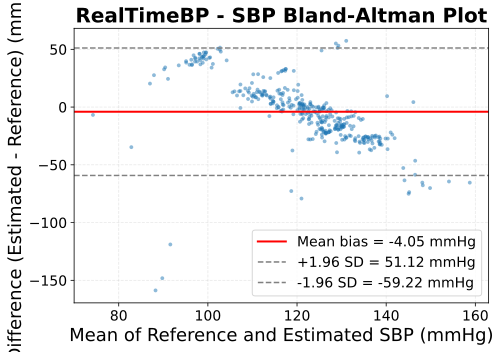
\includegraphics[width=0.32\textwidth]{figures/RealTimeBP_SBP_bland_altman.png}
\hfill
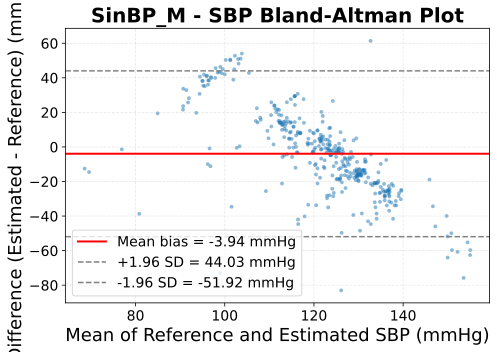
\includegraphics[width=0.32\textwidth]{figures/SinBP_M_SBP_bland_altman.png}
\hfill
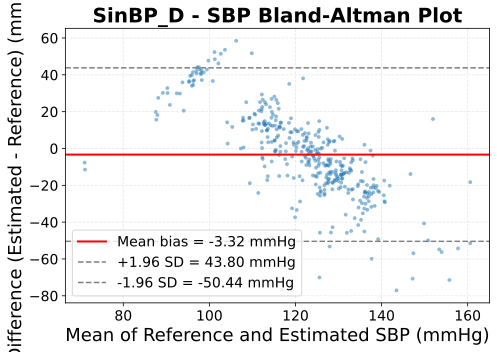
\includegraphics[width=0.32\textwidth]{figures/SinBP_D_SBP_bland_altman.png}
\caption{Bland--Altman plots for SBP. Left: RTBP, Center: sinBP(M), Right: sinBP(D).}
\label{fig:sbp_ba_all}
\end{figure*}

\begin{figure*}[t]
\centering
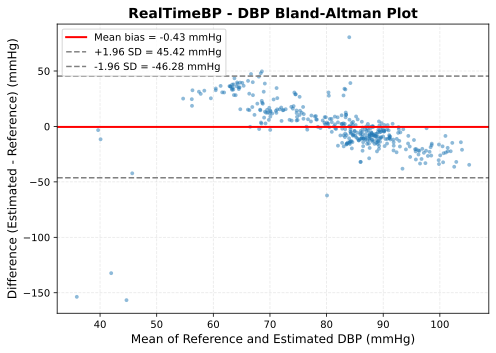
\includegraphics[width=0.32\textwidth]{figures/RealTimeBP_DBP_bland_altman.png}
\hfill
\includegraphics[width=0.32\textwidth]{figures/SinBP_M_DBP_bland_altman.png}
\hfill
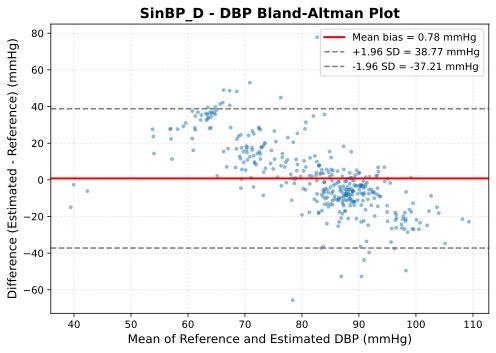
\includegraphics[width=0.32\textwidth]{figures/SinBP_D_DBP_bland_altman.png}
\caption{Bland--Altman plots for DBP. Left: RTBP, Center: sinBP(M), Right: sinBP(D).}
\label{fig:dbp_ba_all}
\end{figure*}

\begin{figure}[t]
\centering
\includegraphics[width=0.49\linewidth]{figures/comparison_SBP_barplot_MAE.png}
\hfill
\includegraphics[width=0.49\linewidth]{figures/comparison_SBP_barplot_RMSE.png}
\\[0.5em]
\includegraphics[width=0.49\linewidth]{figures/comparison_SBP_barplot_MAPE.png}
\caption{SBP accuracy comparison (RTBP, sinBP(M), sinBP(D)). Top-left: MAE, Top-right: RMSE, Bottom: MAPE.}
\label{fig:sbp_comp}
\end{figure}

\begin{figure}[t]
\centering
\includegraphics[width=0.49\linewidth]{figures/comparison_DBP_barplot_MAE.png}
\hfill
\includegraphics[width=0.49\linewidth]{figures/comparison_DBP_barplot_RMSE.png}
\\[0.5em]
\includegraphics[width=0.49\linewidth]{figures/comparison_DBP_barplot_MAPE.png}
\caption{DBP accuracy comparison (RTBP, sinBP(M), sinBP(D)). Top-left: MAE, Top-right: RMSE, Bottom: MAPE.}
\label{fig:dbp_comp}
\end{figure}

Feature Contributions in sinBP(D):
The distortion index $E$ exhibited large positive coefficients (SBP: $+14.88$, DBP: $+15.20$), implying that greater waveform distortion is associated with higher BP---consistent with the physiological link between arteriosclerosis, increased vascular resistance, and waveform distortion. In contrast, $\text{Stiffness}_{\text{sin}}$ ($E\sqrt{A}$) showed negative coefficients (SBP: $-2.40$, DBP: $-3.44$), suggesting that the amplitude-weighted term provides a corrective effect.

Feature Contributions in sinBP(M):
Phase $\Phi$ had positive coefficients (SBP: $+11.79$, DBP: $+15.69$), confirming its significant contribution to BP estimation and reflecting the close relationship between pulse-wave timing and blood pressure.

%-----------------------------------------------------------------------

\section{Discussion}

\subsection{Interpretation of Results}
These results strongly support the effectiveness of the asymmetric sine wave model approximation in a 30\,fps low-sampling-rate environment without relying on frequency analysis.

The improved waveform accuracy (lower MAPE) of sinWave over the raw Green channel demonstrates that the model acts as a noise-removal and waveform-shaping filter, extracting the fundamental PPG component. Model fitting regresses the signal toward a physiologically plausible ``ideal waveform,'' thereby improving the signal-to-noise ratio.

The superior accuracy of sinBP(D) indicates that \emph{deviation from the physiological model} (residual) carries important BP-related information. Quantifying this ``distortion'' and incorporating it as a feature captures subtle physiological changes---such as vascular stiffness and peripheral resistance---that pure parameterization (sinBP(M)) cannot.

\subsection{Superiority of the Proposed Method}
RTBP relies on ``point'' information (peaks, valleys) and is therefore sensitive to sampling jitter at 30\,fps. In contrast, sinBP methods perform least-squares fitting over an entire beat, inherently smoothing timing errors. This robustness explains why sinBP(M) and sinBP(D) outperform RTBP.

Furthermore, sinBP(D) outperforming sinBP(M) demonstrates the value of the ``physiological constraint'' imposed by the asymmetric model. The residual $E$, derived from a model that respects systolic/diastolic asymmetry, more purely reflects pathological or physiological distortion (e.g., vascular stiffening) than simple parameter extraction.

\subsection{Limitations and Future Work}
MAPE remains around 16\%, short of AAMI criteria. Future work should address (1) individual calibration, (2) model extensions (e.g., second-harmonic terms), and (3) larger, more diverse datasets.

%-----------------------------------------------------------------------

\section{Conclusion}
We proposed a blood pressure estimation method based on an asymmetric sine wave model optimized for 30\,fps visible-camera PPG. Experiments showed that sinBP(D), which leverages model residuals, achieved the highest accuracy, confirming the effectiveness of the distortion index as a vascular-stiffness indicator.

The main contribution is an ``asymmetric sine wave model fitting method'' enabling stable feature extraction in low-quality 30\,fps video. Unlike point-based RTBP, this approach exploits the entire waveform shape for improved noise robustness.

This method is expected to contribute to the mHealth field as a convenient blood pressure monitoring technology requiring no dedicated devices. Future work will pursue individual-difference calibration and validation on larger datasets toward practical deployment.

%%%%%%%%%%%%%%%%% BIBLIOGRAPHY IN THE LaTeX file !!!!! %%%%%%%%%%%%%%%%%%%%%%
\begin{thebibliography}{16}
\bibitem{ref1}
World Health Organization. ``Global report on hypertension 2023: the race against a silent killer.'' Geneva: World Health Organization, 2023.

\bibitem{ref2}
Whelton, Paul K., et al. ``2017 ACC/AHA Guideline for the Prevention, Detection, Evaluation, and Management of High Blood Pressure in Adults.'' \textit{Journal of the American College of Cardiology}, vol. 71, no. 19, 2018, pp. e127--e248.

\bibitem{ref3}
Sun, Yu, and Nitish Thakor. ``Photoplethysmography revisited: from contact to noncontact, from point to imaging.'' \textit{IEEE Transactions on Biomedical Engineering}, vol. 63, no. 3, 2016, pp. 463--477.

\bibitem{ref4}
Allen, John. ``Photoplethysmography and its application in clinical physiological measurement.'' \textit{Physiological Measurement}, vol. 28, no. 3, 2007, pp. R1--R39.

\bibitem{ref5}
Millasseau, Sandrine C., et al. ``Contour analysis of the photoplethysmographic pulse measured at the finger.'' \textit{Journal of Hypertension}, vol. 24, no. 8, 2006, pp. 1449--1456.

\bibitem{ref6}
Nichols, Wilmer W. ``Clinical measurement of arterial stiffness obtained from noninvasive pressure waveforms.'' \textit{American Journal of Hypertension}, vol. 18, no. 1, 2005, pp. 3S--10S.

\bibitem{ref7}
Charlton, Peter H., et al. ``Assessing model age from the photoplethysmogram: a systematic review.'' \textit{IEEE Reviews in Biomedical Engineering}, vol. 12, 2019, pp. 179--202.

\bibitem{ref8}
Elgendi, Mohamed. ``On the analysis of fingertip photoplethysmogram signals.'' \textit{Current Cardiology Reviews}, vol. 8, no. 1, 2012, pp. 14--25.

\bibitem{ref9}
Alian, Aymen A., and Kirk H. Shelley. ``Photoplethysmography.'' \textit{Best Practice \& Research Clinical Anaesthesiology}, vol. 28, no. 4, 2014, pp. 395--406.

\bibitem{ref10}
Zhang, Liang, et al. ``Developing personalized models of blood pressure estimation from wearable sensors data using minimally-trained domain adversarial neural networks.'' \textit{Proceedings of Machine Learning Research}, vol. 126, 2020, pp. 97--120.

\bibitem{ref11}
Verkruysse, Wim, Lars O. Svaasand, and J. Stuart Nelson. ``Remote plethysmographic imaging of skin perfusion.'' \textit{Optics Express}, vol. 16, no. 26, 2008, pp. 21434--21445.

\bibitem{ref12}
McDuff, Daniel, et al. ``Improvements in remote cardiopulmonary measurement using a five band camera.'' \textit{IEEE Transactions on Biomedical Engineering}, vol. 61, no. 10, 2014, pp. 2593--2601.

\bibitem{ref13}
Basso, G., Haakma, R., and Vullings, R. ``A skewed-Gaussian model for pulse decomposition.'' \textit{Physiological Measurement}, vol. 45, no. 11, 2024.

\bibitem{ref14}
Tiinanen, T., Popa, A.-G., K\"{a}pyl\"{a}, M., and Fr\"{a}nti, A. ``Model selection for the pulse decomposition analysis of fingertip photoplethysmograms.'' \textit{Proc. IEEE Eng. Med. Biol. Soc. (EMBC)}, 2017, pp. 1624--1627.

\bibitem{ref15}
Mukkamala, Ramakrishna, et al. ``Toward ubiquitous blood pressure monitoring via pulse transit time: theory and practice.'' \textit{IEEE Transactions on Biomedical Engineering}, vol. 62, no. 8, 2015, pp. 1879--1901.

\bibitem{ref16}
Hall, John E., and Michael E. Hall. \textit{Guyton and Hall Textbook of Medical Physiology}. 14th ed., Elsevier, 2020.
\end{thebibliography}

\end{document}
